\documentclass[tikz, border = 0.2cm]{standalone}
%TikZ and Plots
\usepackage{tikz} 
\usetikzlibrary{shapes.misc,patterns,hobby,decorations.markings, snakes, calc, shadows, fit, backgrounds}
\usepackage{pgfplots}

%Color Settings
\usepackage{xcolor}
\definecolor{MScRed}{RGB}{157,0,0}
\definecolor{MScBlue}{RGB}{1,1,141}
\definecolor{MScGreen}{RGB}{0, 119, 85}
\definecolor{MScGray}{RGB}{102, 102, 142}

%Math and Units
\usepackage{amsmath, amssymb, commath, mathtools}
\usepackage{relsize}
\usepackage{physics}
\usepackage{xfrac}
\usepackage[separate-uncertainty]{siunitx}

%Language Settings and Microtype
\usepackage{fontspec, xunicode}
\usepackage[utf8]{inputenc}
\usepackage{lmodern}
\setmainfont{Palatino}
\setsansfont{Optima}
\setmonofont[Scale=MatchLowercase]{Menlo}

\usetikzlibrary{decorations.pathreplacing}

\tikzset{invclip/.style={clip,insert path={{[reset cm]
      (-\maxdimen,-\maxdimen) rectangle (\maxdimen,\maxdimen)
    }}}}
    
\begin{document}

\begin{tikzpicture}
%\draw[help lines] (-2,0) grid (12,10); 


%Steps
\node[draw, ultra thick, drop shadow, rounded corners, fill = white, black , text=black, minimum size = 2cm ] at (5, 9) {\quad\Large{1. Choose appropriate initial spectral functions $\rho_{q, \text{init}}^{(D/M)}$\phantom{\quad}}};

\node[draw, ultra thick, drop shadow, rounded corners, fill = white, black , text=black, minimum size = 2cm ] at (5, 5) {\quad\Large{2. Compute} 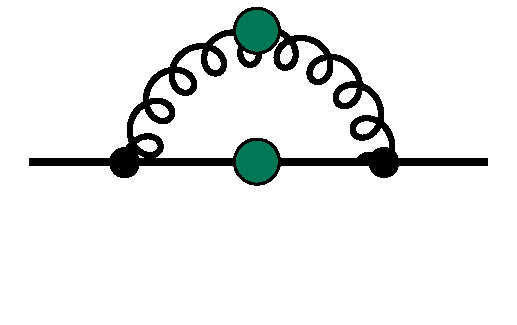
\includegraphics[scale=0.25, trim= 0 1.3em 0 0]{diagram} \Large{employing the updated spectral functions\phantom{\quad}}};

\node[draw, ultra thick, drop shadow, rounded corners, fill = white, black , text=black, minimum size = 2cm ] at (5, 1) {\quad\Large{3. Access $\Gamma^{(2)}_q$ and the propagator dressings $M_q$ and $Z_q$ via the DSE\phantom{\quad}}};

\node[draw, ultra thick, drop shadow, rounded corners, fill = white, black , text=black, minimum size = 2cm ] at (5, -3) {\quad\Large{4. Extract $\rho_q^{(D/M)}$ from the respective  propagator dressings\phantom{\quad}}};

%Arrows and description
\draw[ultra thick,MScRed, ->] (5,7.8) to (5,6.2);
\draw[ultra thick,MScRed, ->] (5,3.8) to (5,2.2);
\draw[ultra thick,MScRed, ->] (5,-0.2) to (5,-1.8);

\draw[ultra thick, MScRed, ->] (-2.5, -3) to[out=150,in=190] (-3.2,5);
\node[text width = 3cm, align = center, MScRed] at (-7, 1) {\Large Feed back\\[0.5em] into the DSE};

\draw [ultra thick, text width = 3cm, align = center, decorate, decoration={brace,amplitude=10pt,mirror, raise=-40pt}, yshift=0pt]
(15,-4) -- (15,6) node [black,midway,xshift=0.8cm] {\Large
Iterate until\\[0.5em] convergence};

\end{tikzpicture}
\end{document} 